\chapter{Feature Extraction}
\label{ch:FeatureExtraction}

Before diving into the novelty detection framework itself, the features to be used need to be defined and extracted from the data. Since our goal is to detect a novel behavior, we are interested in both \quoted{time-domain} and \quoted{frequency-domain} features. The former are used to capture the temporal evolution of the signal, while the latter are used to capture the spectral content of the signal. 
In this chapter, we will first introduce the reference dataset that will be used to test the framework and then we will describe the features that will be used in the framework. The \gls{nd} framework will work on the complete collection of features $\vect{F}=\{\vect{F}_t, \vect{F}_f\}$, where $\vect{F}_t$ is the collection of time-domain features and $\vect{F}_f$ is the collection of frequency-domain features. Some of the features will be extracted for all the signals available, while some others only on a subset of the signals, depending on the settings of the framework, as it will be explained in \autoref{ch:Framework}. 



\section{Reference dataset}
In the field of \gls{nd}, a famous bearing vibration dataset has been collected from the Center for Intelligent Maintenance Systems (\gls{ims}) of the University of Cincinnati and made available online on the \gls{nasa} website \cite{lee2007bearingdataset}. 
Let's take this as a starting point for our work. The dataset contains the vibration measurements collected at a sampling frequency $f_s=20\si{\kHz}$ of four forced-lubricated bearings. The shaft was kept constant at $2000$rpm during the data collection. The test rig is shown in \autoref{fig:IMS_bearing_dataset} and the test parameters are summarized in \autoref{tab:IMS_test_parameters}, which also shows the type of faults that happened in each repetition of the test.

To visualize what happens to the vibration signal as the bearing degrades over time, let's consider the \quoted{Bearing 3 x} signal from the \gls{ims} dataset, shown in \autoref{fig:IMS_bearing}. The top plot shows the vibration of the new bearing, while the bottom plot shows the vibration of the bearing just before the test was stopped. It's evident that the degraded signal reaches greater peaks in vibration and has a greater variance. The narrow peaks in the degraded signal are due to the presence of fault frequencies, that are not present in the new bearing signal.

\begin{figure}
    \centering
    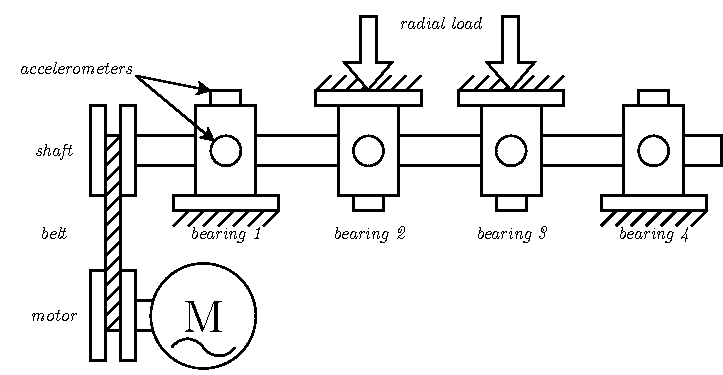
\includegraphics[scale=1]{images/FeatureExtraction/testrig.pdf}
    \caption{The test rig used by \cite{lee2007bearingdataset}}
    \label{fig:IMS_bearing_dataset}
\end{figure}

\begin{figure}
    \centering
    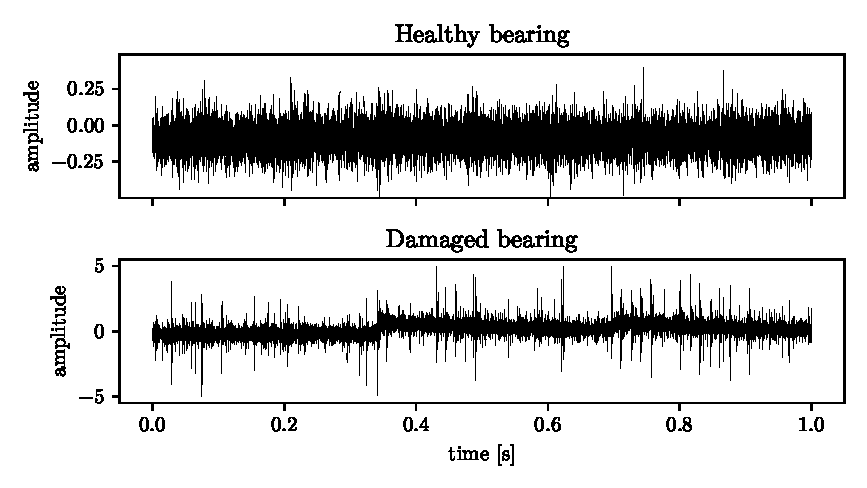
\includegraphics[scale=1]{images/FeatureExtraction/TD_signal.pdf}
    \caption{\quoted{Bearing 3 x} vibration signal from the \gls{ims} dataset}
    \label{fig:IMS_bearing}
\end{figure}

% \usepackage{tabularray}
\begin{table}
    \centering
    \caption{Test setup \cite{lee2007bearingdataset}}
    \label{tab:IMS_test_parameters}
    \resizebox{\linewidth}{!}{%
    \begin{tblr}{
      cell{2}{1} = {t},
      cell{2}{2} = {t},
      cell{3}{1} = {t},
      cell{3}{2} = {t},
      cell{5}{1} = {t},
      cell{5}{2} = {t},
      cell{6}{1} = {t},
      cell{6}{2} = {t},
      cell{7}{1} = {t},
      cell{7}{2} = {t},
      hline{1,8} = {-}{0.08em},
      hline{2} = {-}{},
    }
     & \textbf{Set No. 1} & \textbf{Set No. 2} & \textbf{Set No. 3}\\
    \textbf{Recording Duration} & 22/10/2003 - 25/11/2003 & 12/02/2004 - 19/02/2004 & 04/03/2004 - 04/04/2004\\
    \textbf{No. of Files} & 2156 & 984 & 4448\\
    \textbf{No. of Channels} & 8 & 4 & 4\\
    \textbf{Channel Arrangement} & {Bearing 1 ch 1  2\\Bearing 2 ch 3  4
    \\Bearing 3 ch 5  6
    \\Bearing 4 ch 7 \& 8~ ~~} & {Bearing 1 ch 1\\Bearing 2 ch 2\\Bearing 3 ch 3\\Bearing 4 ch 4 ~} & {Bearing 1 ch 1\\Bearing 2 ch 2\\Bearing 3 ch 3\\Bearing 4 ch 4~ ~~}\\
    \textbf{File Recording Interval} & 5 or 10 min & 10 min & 10 min\\
    \textbf{Fault type } & {Bearing 3: inner race defect\\Bearing 4: roller element defect} & Bearing 1: outer race failure & Bearing 3: outer race failure
    \end{tblr}
    }
    \end{table}

\section{Time-domain features}
Let's consider a timeserie $\vect{x}$ containing $n$ samples $x_1, x_2, \dots, x_n$. The goal of the feature extraction process is to extract a set of features $\vect{F}_t = \{F_1, F_2, \dots, F_m\}$ that can be used to describe the signal. In this section, we will describe the features that will be used in the developed framework.
\paragraph{Mean}
The first feature to be considered is simply the mean of the signal. It is defined as
\begin{equation}
    \mu = \frac{1}{n}\sum_{i=1}^n x_i
\end{equation}

\paragraph{\gls{rms}}
The Root mean square of the signal \gls{rms} is related to the power and is defined as
\begin{equation}
    \text{RMS} = \sqrt{\frac{1}{n}\sum_{i=1}^n x_i^2}
\end{equation}

\paragraph{Peack-to-peak}
The peak-to-peak value of the signal is defined as
\begin{equation}
    \text{P2P} = \max(\vect{x}) - \min(\vect{x})
\end{equation}

\paragraph{Standard deviation}
The standard deviation is a measure of the dispersion of the signal and is defined {\gls{wrt}} a known distribution with knowledge of the true mean $\mu_{true}$ as

\begin{equation}
    {\sigma} = \sqrt{\frac{1}{n}\sum_{i=1}^n (x_i - \mu_{true})^2}
\end{equation}

but since in our case we don't know the true mean, we will use the sampled standard deviation, which is the best estimate, defined as

\begin{equation}
    \hat{\sigma} = \sqrt{\frac{1}{n-1}\sum_{i=1}^n (x_i - \mu)^2}
\end{equation}

\paragraph{Skewness}
The skewness is a measure of the asymmetry of the signal and is defined as
\begin{equation}
    \gamma = \gls{sym:E}\left[ \left(\frac{x - \mu}{\sigma}\right)^3 \right]
\end{equation}

and can be estimated on sampled data as

\begin{equation}
  \hat{\gamma} = \frac{\sqrt{n(n-1)}}{n-2} \frac{\tfrac{1}{n} \sum_{i=1}^n (x_i-\overline{x})^3}{\left[\tfrac{1}{n} \sum_{i=1}^n (x_i-\overline{x})^2 \right]^{3/2}}
\end{equation}

\paragraph{Kurtosis}
The kurtosis is a measure of the \quoted{peakedness} of the signal and is defined as
\begin{equation}
    \kappa = \frac{1}{n}\sum_{i=1}^n \left(\frac{x_i - \mu_{true}}{\sigma}\right)^4
\end{equation}

and can be estimated on sampled data as

\begin{equation}
  \hat{\kappa} = \frac{(n+1)\,n}{(n-1)\,(n-2)\,(n-3)} \; \frac{\sum_{i=1}^n (x_i - \mu)^4}{k_2^2} - 3\,\frac{(n-1)^2}{(n-2) (n-3)}
\end{equation}

\begin{figure}
    \centering
    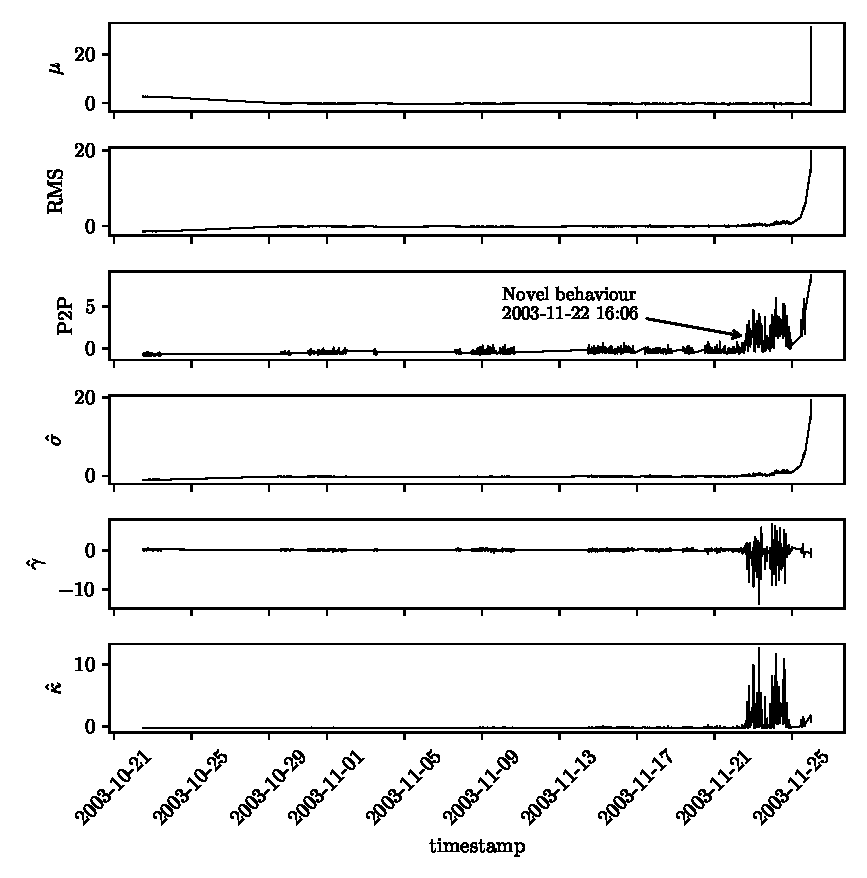
\includegraphics[scale=1]{images/FeatureExtraction/TDfeatures.pdf}
    \caption{All time-domain features for the \quoted{Bearing 3 x} vibration signal from the \gls{ims} dataset}
    \label{fig:IMS_TD_features}
\end{figure}

To visualize the evolution of the features over time, let's consider all the snapshots of the \quoted{Bearing 3 x} signal from the \gls{ims} dataset and plot all the time-domain features described above. The result is shown in \autoref{fig:IMS_TD_features}. Having seen also \autoref{fig:IMS_bearing}, it's not surprising that the P2P and the kurtosis are the time domain features that capture the degradation of the bearing the earliest. 


\section{Frequency-domain features}

To capture also the frequency behavior of the signal, other tools are needed. In this section, we will describe the frequency-domain features  $\vect{F}_f = \{F_{m+1}, F_{m+2}, \dots, F_l\}$ that will be used in the developed framework.

\subsection{Fourier Transform}
\label{sec:FFT}

One powerful tool to analyze the frequency content of a signal is the Fourier transform or, in the case of a discrete signal, the Discrete Fourier Transform(\gls{dft}), which has a very efficient implementation in the Fast Fourier Transform (\gls{fft}) algorithm \cite{cooley1965algorithm}. This algorithm is implemented in many programming languages and libraries, including \texttt{python} and \texttt{C}. The theory behind this topic is briefly described in \autoref{app:FFT}. 

To have a better understanding of the capability of the \gls{fft} to capture the frequency content of a signal (and the presence of a disturbance in a portion of the signal), let's consider the following signal, composed by the sum of four sinusoids with different frequencies that is plotted with its \gls{dft} in \autoref{fig:FD_known}:
\begin{multline}
    x(t) = \sin(2\pi f_1 t) + \sin(2\pi f_2 t) + \sin(2\pi f_3 t) + \sin(2\pi f_4 t), \\
    t \in [0, 1], \quad \{f_1, f_2, f_3, f_4\} = \{2, 5, 7, 15\} \si{\Hz}
\end{multline}

In the \autoref{fig:FD_known} it is possible to see the four peaks in the frequency domain, corresponding to the four frequencies of the sinusoids. Now, let's consider the same signal, but with an additive disturbance in a small portion of the signal, as shown in \autoref{fig:FD_known_dist}. The disturbance is a period of the signal $x(t) = \sin(2\pi f_5 t)$, with $f_5=50\si{\Hz}$, that is added to the signal in the interval $t \in [0.4, 0.6]$. The \gls{dft} of this signal is shown in \autoref{fig:FD_known_dist}. It is possible to see that the disturbance is captured by the spectrum as a broad frequency additional components, instead of a peak at $f_5=50\si{\Hz}$. This is because the disturbance is not acting on the whole signal. For our purpose, this is still good because we can detect the variation of all the frequencies involved.

Consider the period of the undisturbed signal, that is the \gls{lcm} of the periods of the four sinusoids composing the signal.
\[ 
    T = \text{LCM} \left( \frac{1}{2} \si{\s},\frac{1}{5}\si{\s},\frac{1}{7}\si{\s},\frac{1}{15}\si{\s} \right) = 1 \si{\s}
\]

So, we were processing a signal that has a period of one second, sampled for exactly one second. Let's see what happens if we sample the same signal for a time that is not an integer multiple of the period. In \autoref{fig:FD_known_leackage} it is shown the \gls{dft} of the same signal as before, but sampled for $t \in [0, 0.9]$. It is possible to see that the peaks are still at the frequencies of the sinusoids composing the signal, but they are not single points as it appears that also frequencies near the true frequencies are present. This phenomenon is called \emph{spectral leackage} and happens because the signal is not sampled for an integer number of periods \cite{SpectralLeakage}. 


\begin{figure}
    \centering
    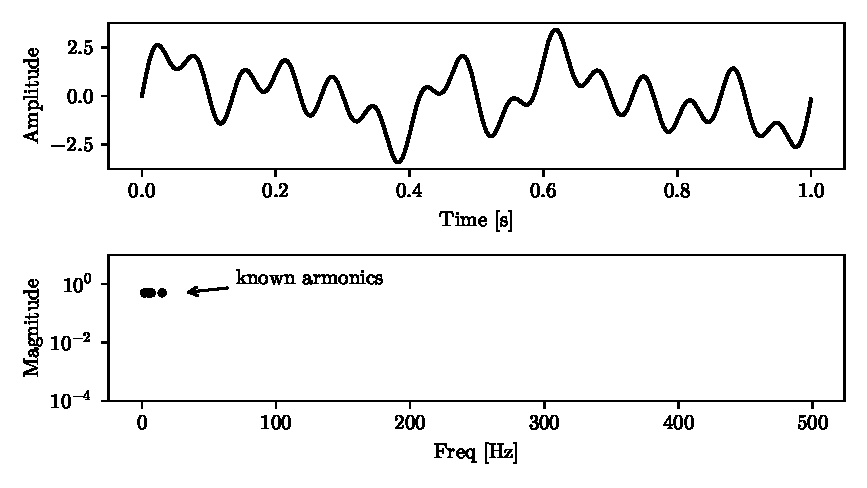
\includegraphics[scale=1]{images/FeatureExtraction/FD_known.pdf}
    \caption{FFT of the signal with known frequency components}
    \label{fig:FD_known}
\end{figure}

\begin{figure}
    \centering
    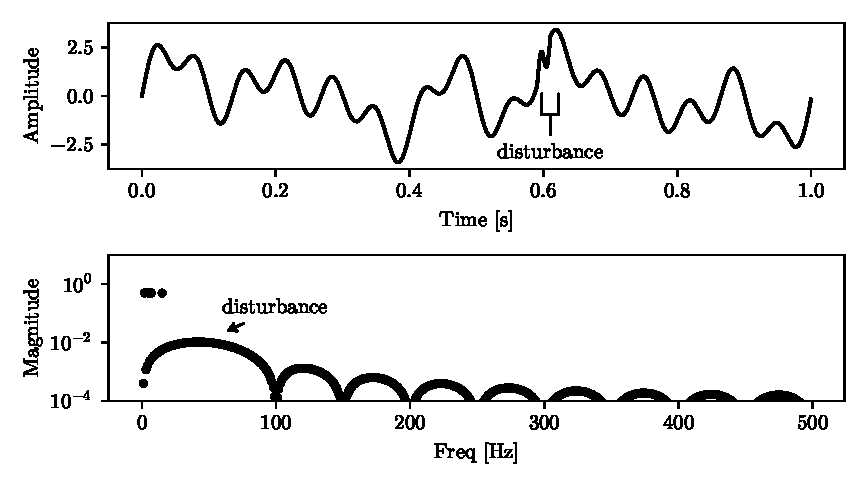
\includegraphics[scale=1]{images/FeatureExtraction/FD_known_dist.pdf}
    \caption{FFT of the signal with known frequency components, and an additive disturbance}
    \label{fig:FD_known_dist}
\end{figure}

\begin{figure}
    \centering
    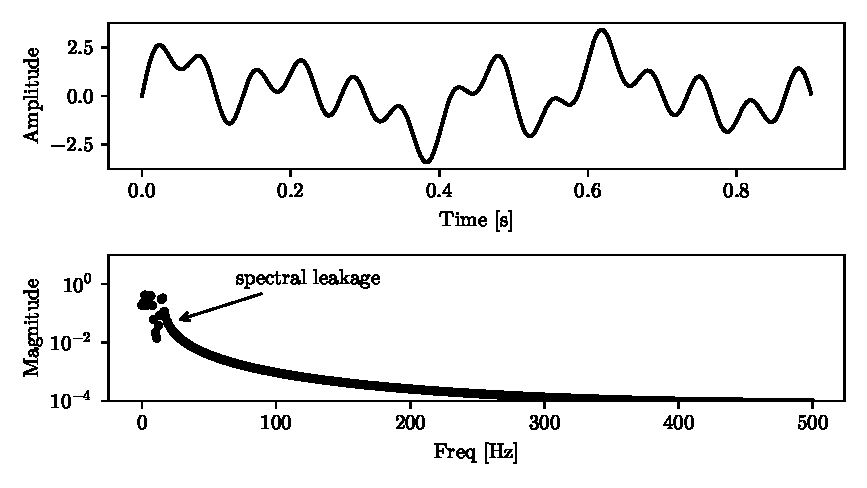
\includegraphics[scale=1]{images/FeatureExtraction/FD_known_outofsync.pdf}
    \caption{FFT of the signal with known frequency components, with a domain that is not an integer multiple of the period}
    \label{fig:FD_known_leackage}
\end{figure}

\begin{figure}
    \centering
    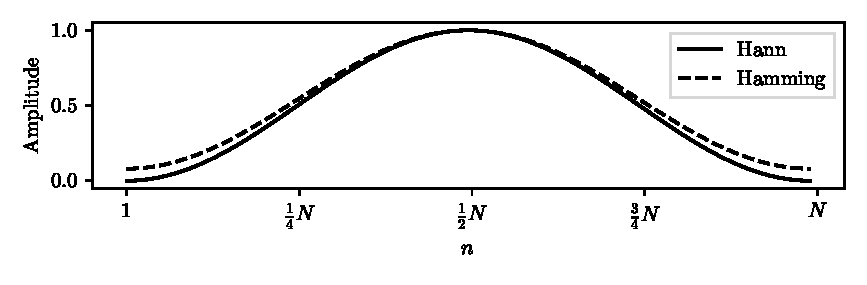
\includegraphics[scale=1]{images/FeatureExtraction/windows.pdf}
    \caption{Hann and Hamming windows}
    \label{fig:windows}
\end{figure} 


\subsubsection{Preprocessing}
Up to now, it has been shown that the \gls{dft} will translate the presence of a disturbance in the time domain into several periodic components in the frequency domain. However, it has the spectral leakage weakness if the sampling interval is not an integer multiple of the period of the signal which is the most likely scenario in a real application. To compensate for this phenomenon, it is better to use a transformation to the signal that makes it artificially start and end with the same value. This can be done with a \emph{windowing} function, or with the \emph{flip and reverse} method \cite{Preprocessing}. 

The most common windowing funcitons are the \emph{Hann} and the \emph{Hamming} windows, defined as:
\begin{eqnarray}
    w_{hann}(i) = 0.5\; \left[1 - \cos \left ( \frac{2 \pi i}{n} \right) \right] \\
    w_{hamming}(i) = \frac{25}{46}\; \left[1 - \cos \left ( \frac{2 \pi i}{n} \right) \right]
\end{eqnarray}
where $i$ is the considered sample as independent variable and $n$ is the total number of samples. Those functions are plotted in \autoref{fig:windows}. The preprocessing operation is simply to multiply the signal by the windowing function. this will make the first and last point of the signal exactly zero in the case of the Hann window, and very close to zero in the case of the Hamming window but with the advantage of having a narrower peak in the spectrum. 

The \quoted{flip and reverse} method is simply to concatenate a flipped copy of the signal to itself and downsampling it to preserve the original length of the array, as follows \cite{Preprocessing}:

\begin{equation}
    x_{new}(i) = \begin{cases}
        x(2i) & \text{if } i \leq \frac{n}{2} \\
        x(2(n-i)) & \text{if } i > \frac{n}{2}
    \end{cases} \qquad \forall i \in [1,n]
\end{equation}

A comparison of those preprocessing techniques is shown in \autoref{fig:FD_preprocessing} and \autoref{fig:FD_preprocessing_dist}. In both figures, it is evident that the \quoted{flip and reverse} method generates a fake peak at half the sampling frequency, while the windowing function doesn't. Moreover, looking at \autoref{fig:FD_preprocessing_dist}, it is possible to see that the Hann window better suppresses the spectral leakage.
In figure \autoref{fig:IMS}, it is shown the effect of different preprocessing techniques on a real-world signal from the \gls{ims} dataset. The Hann window will be implicitly used in the rest of this section.



\begin{figure}
    \centering
    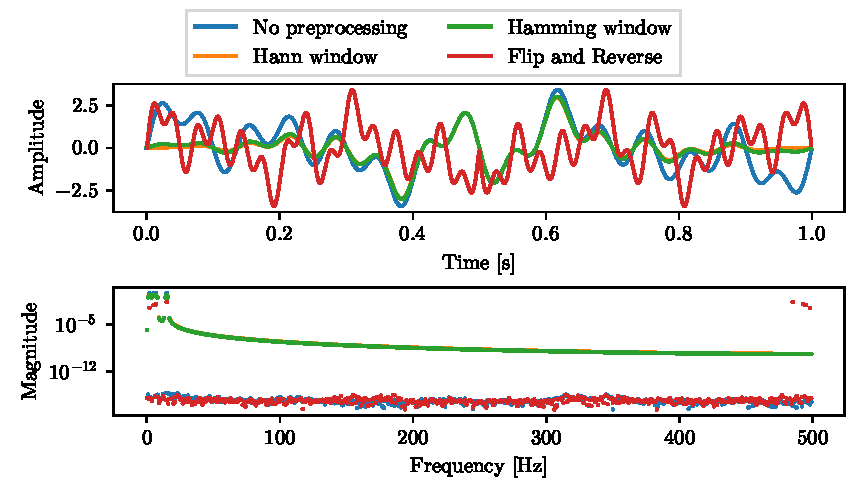
\includegraphics[scale=1]{images/FeatureExtraction/FD_Preproc_sync.pdf}
    \caption{FFT of the signal  with a domain that is an integer multiple of the period, and preprocessing techniques applied}
    \label{fig:FD_preprocessing}
\end{figure}

\begin{figure}
    \centering
    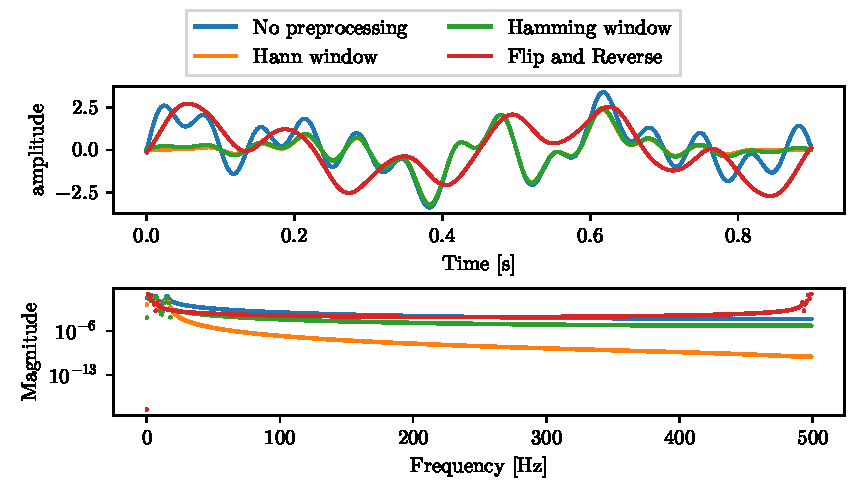
\includegraphics[scale=1]{images/FeatureExtraction/FD_Preproc_outofsync.pdf}
    \caption{FFT of the signal with a domain that is not an integer multiple of the period, and preprocessing techniques applied}
    \label{fig:FD_preprocessing_dist}
\end{figure}

\begin{figure}
    \centering
    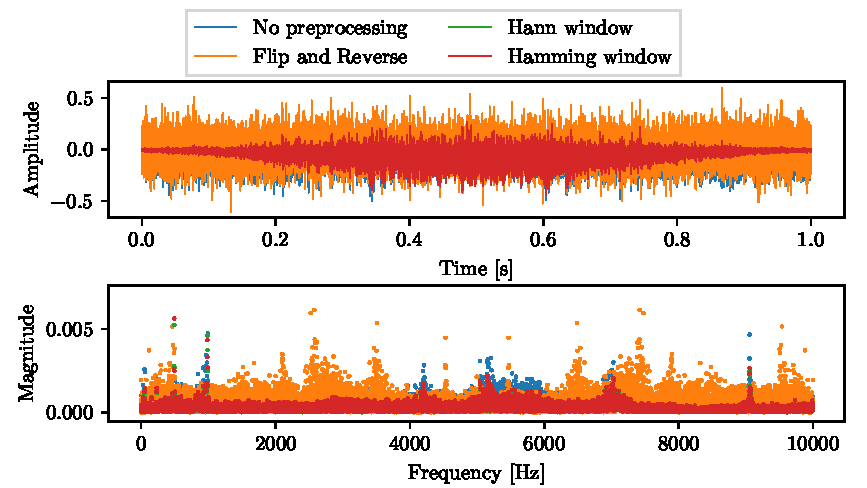
\includegraphics[scale=1]{images/FeatureExtraction/FD_PreprocIMS.pdf}
    \caption{FFT of the \quoted{Bearing 3 x} vibration signal from the \gls{ims} dataset, in normal conditions, with preprocessing techniques applied}
    \label{fig:IMS}
\end{figure}


\subsubsection{Application to the reference dataset}

At this point, to see if the spectrum is representative of a fault, as it has been done for the time-domain features, we can plot all the spectrum for all the snapshots of the \quoted{Bearing 3 x} signal from the \gls{ims} dataset, as shown in \autoref{fig:IMS_FD}. Looking at the picture, we can see that the signature frequencies of faults are present in the spectrum, and they become more and more prominent as the bearing degrades. This is a good sign justifying to use of the spectrum to detect the novel behaviour.

\begin{figure}
    \centering
    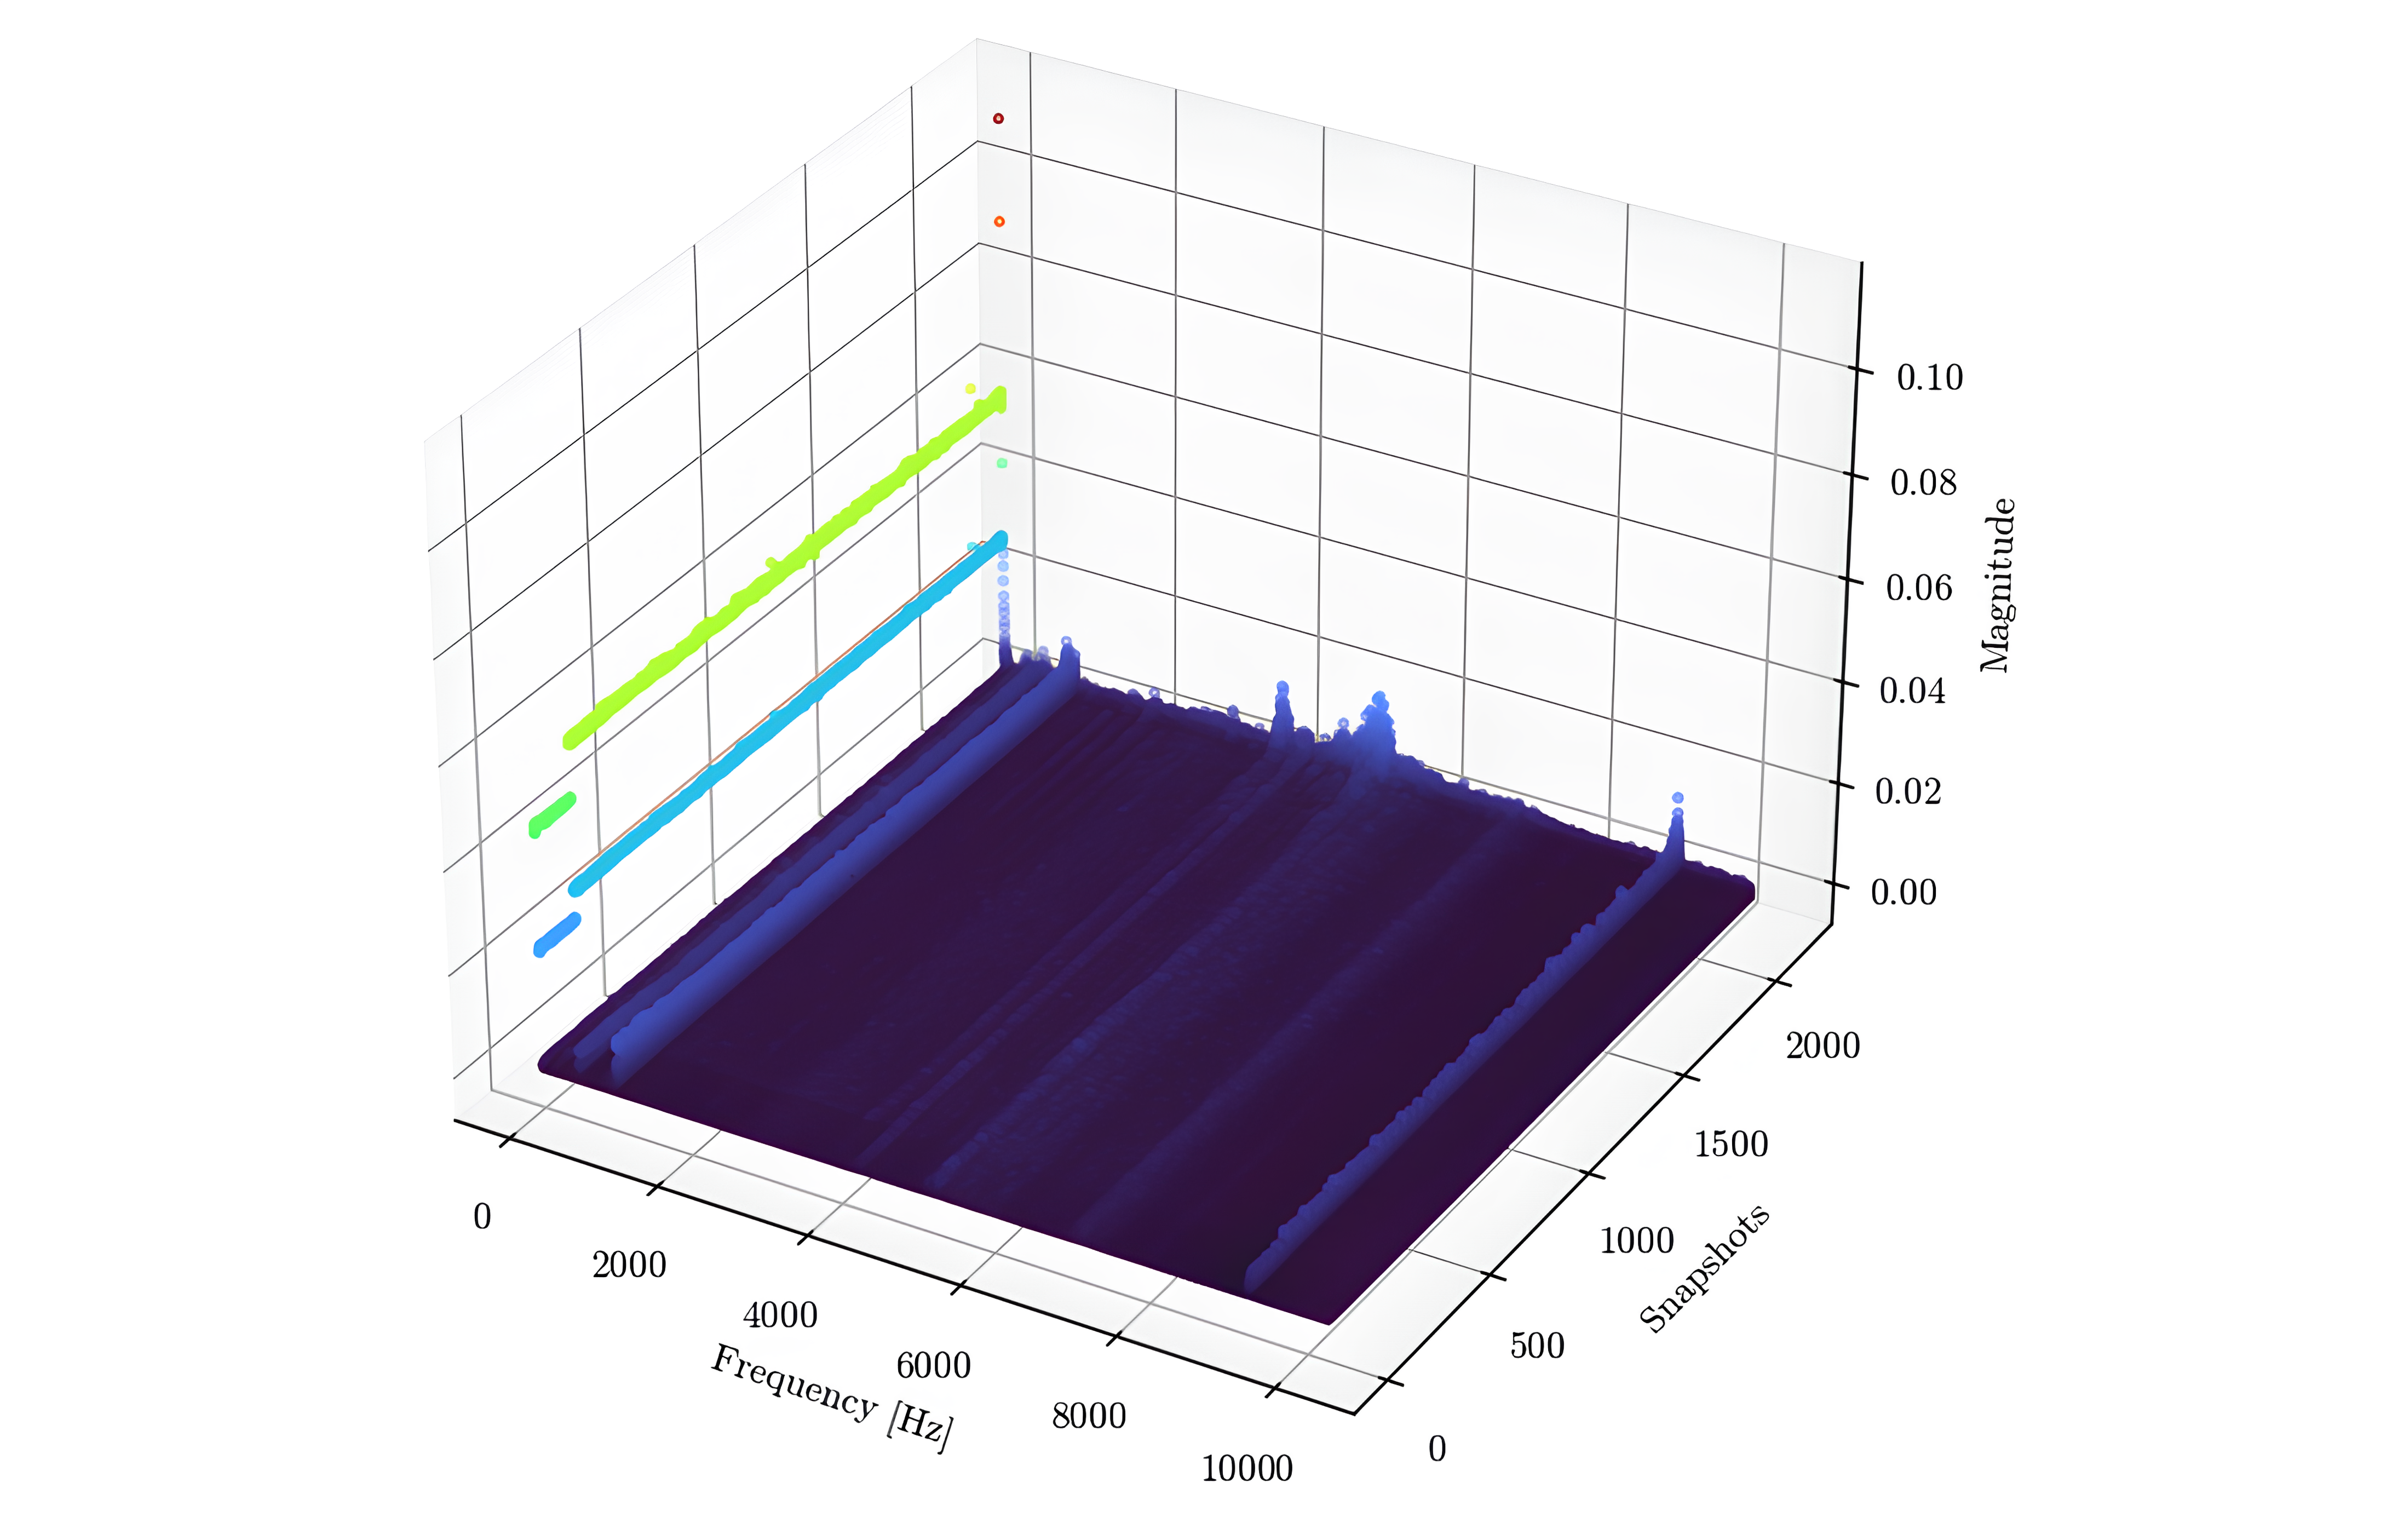
\includegraphics[width=\textwidth]{images/FeatureExtraction/FD_IMS.png}
    \caption{FFT of the \quoted{Bearing 3 x} vibration signal from the \gls{ims} dataset, in normal conditions with hann window preprocessing
    applied}
    \label{fig:IMS_FD}
\end{figure}


\subsection{Wavelet Packet Decomposition}
\label{sec:WPD}

\subsubsection{Motivation}

In the previous \autoref{sec:FFT}, it has been shown that the spectrum of the signal contains useful information for performing \gls{nd}. Remembering that the ultimate scope of this work is to develop a framework that runs in \gls{glo:edge}, it is important to consider the computational cost of the features extraction, and the memory usage. Considering only the \gls{fft} of all signal of the dataset shown in \autoref{fig:IMS_FD} and the fact that a floating point value uses $64$ bit, the memory usage is $64 \si{\bit} \times 10 \text{kFeatures} \times 2156 \text{Snapshots} \div 8 \text{bit/byte} \approx 172.5 \text{Mb}$. This is not a big problem for a desktop computer, but it may be a problem for an \gls{iot} device. Moreover, the \gls{fft} is a very computationally expensive operation, with a complexity of $\mathcal{O}(n \log n)$, where $n$ is the number of samples.

To overcome this problem it is necessary to find a method that exploits the same information in the frequency domain, but using much less computational power and memory. Other tools for the frequency analysis are the Wavelet Transform, and in particular the Wavelet Packet Decomposition (\gls{wpd}) has been used in the developed framework. The theory behind this topic is briefly described in \autoref{app:wavelet}.

\subsubsection{Application to the reference dataset}

At this point, let's consider a \gls{wpd} with a dept of $6$, that outputs $2^6=64$ coefficients. We are going to take the norm of each coefficient as a feature so, in the end, we will have $64$ features (from \quoted{aaaaaa} that is lead from all the approximation coefficients to \quoted{dddddd} that that is lead from all the detail coefficients instead, passing for all the combinations in between). The \gls{wpd} of the \quoted{Bearing 3 x} signal from the \gls{ims} dataset is shown in \autoref{fig:IMS_WPD_health} as the bearing is new, and in \autoref{fig:IMS_WPD_fault} as the bearing is degraded. It is possible to see that the \gls{wpd} is able to capture the presence of the fault frequencies.

\begin{figure}
    \centering
    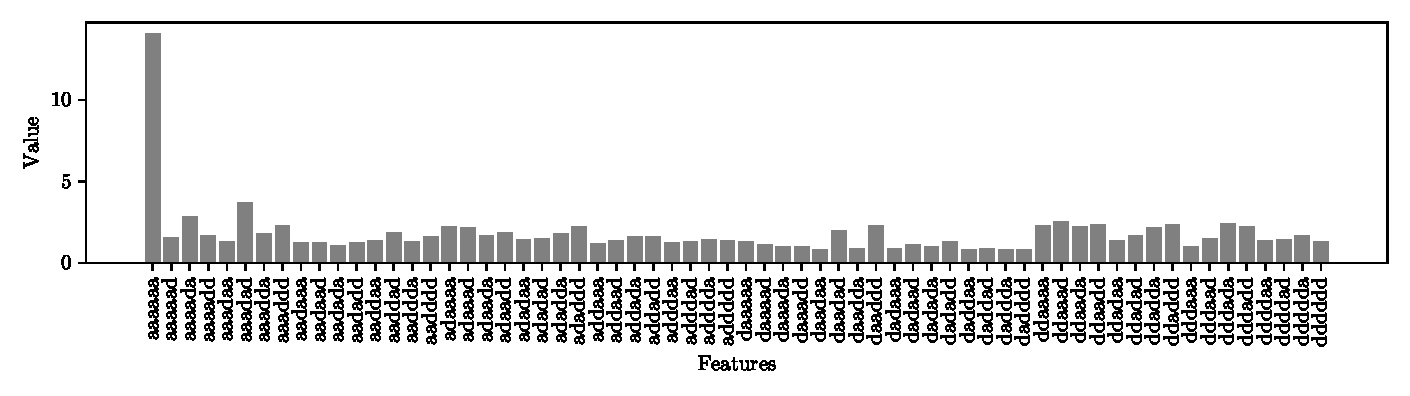
\includegraphics[width=\textwidth]{images/FeatureExtraction/IMS_WPD_health.pdf}
    \caption{Wavelet Packet Decomposition of the \quoted{Bearing 3 x} vibration signal from the \gls{ims} dataset, in normal conditions}
    \label{fig:IMS_WPD_health}
\end{figure}

\begin{figure}
    \centering
    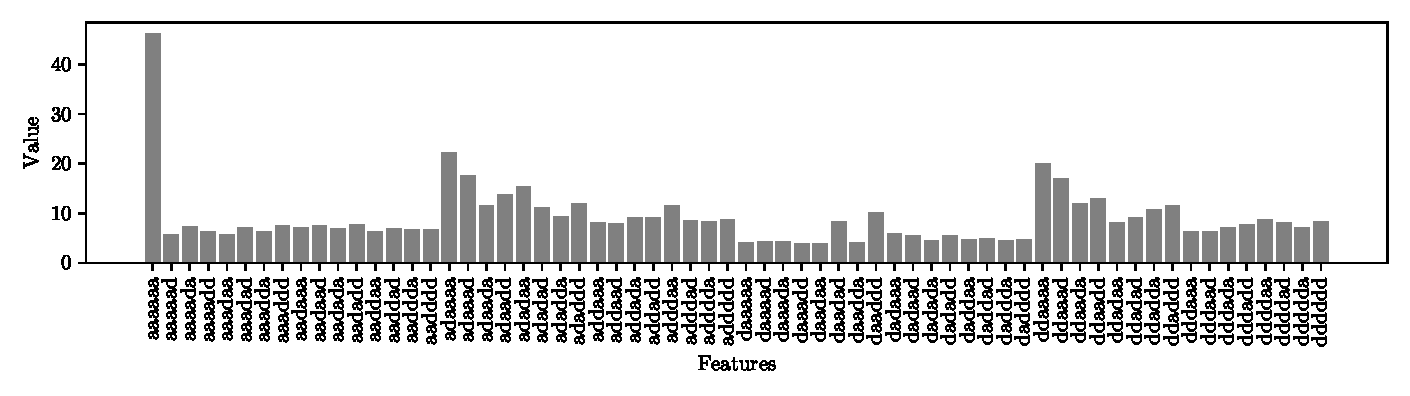
\includegraphics[width=\textwidth]{images/FeatureExtraction/IMS_WPD_fault.pdf}
    \caption{Wavelet Packet Decomposition of the \quoted{Bearing 3 x} vibration signal from the \gls{ims} dataset, in abnormal conditions}
    \label{fig:IMS_WPD_fault}
\end{figure}

At this point, it is possible to extract the features with the \gls{wpd} and plot them over time, for the whole dataset, as it has been done for the \gls{fft} in \autoref{fig:IMS_FD}. The result is shown in \autoref{fig:IMS_WPD}. The memory consumption of the data in the second figure is $64 \si{\bit} \times 64 \text{Features} \times 2156 \text{Snapshots} \div 8 \text{bit/byte} \approx 1.1 \text{Mb}$, that means that the memory saving obtained using \gls{wpd} instead of \gls{fft} exceeds $99\%$. 
Despite this huge memory saving, it is possible to see that the \gls{wpd} is able to retain the information about the fault frequencies, and it is possible to see that the fault frequencies become more and more prominent as the bearing degrades over time. For this reason, the \gls{wpd} will be used in the developed framework, along with the time-domain features.

\begin{figure}
    \centering
    \includegraphics[scale=0.99]{images/FeatureExtraction/WPD_IMS.pdf}
    \caption{Wavelet Packet Decomposition of the \quoted{Bearing 3 x} vibration signal from the \gls{ims} dataset, in normal conditions}
    \label{fig:IMS_WPD}
\end{figure}

\section{Conclusions}
Even just considering very simple time-domain features, we can already detect the degradation of the bearing by comparing these feature values to a threshold. On the other hand, also the frequency-domain features could be just compared with a threshold to detect novel behaviors. But, as we will see in \autoref{ch:Framework}, a general purpose framework based upon a more sophisticated approach based on the clustering of the data, it will be possible to condense all the features from all the signals into a single metric that will be used to detect the novel behavior. This will have several advantages. Some of them are being able to detect a novel behavior even if it is not possible to define a threshold for each feature, and the single threshold to be defined on the metric will be easier to interpret and tune. Moreover, the framework will be able to detect the novelty even earlier and even if the degradation of the bearing is not captured by the time-domain features, but only by the frequency-domain features.

